\section{fulibWorkflows Web-Editor Frontend}\label{sec:editor-frontend}
Nachdem die erste Hälfte der Implementierung durch fulibWorkflows abgeschlossen ist, konzentrieren sich dieses und das folgende Kapitel um den dazugehörigen Web-Editor.
Der Web-Editor besteht aus einem Frontend und einem Backend, welche beide über Heroku deployed wurden und somit erreichbar sind.
Erreichbar ist der Web-Editor unter~\url{https://workflows-editor-frontend.herokuapp.com/}.

\begin{figure}[h]
    \centering
    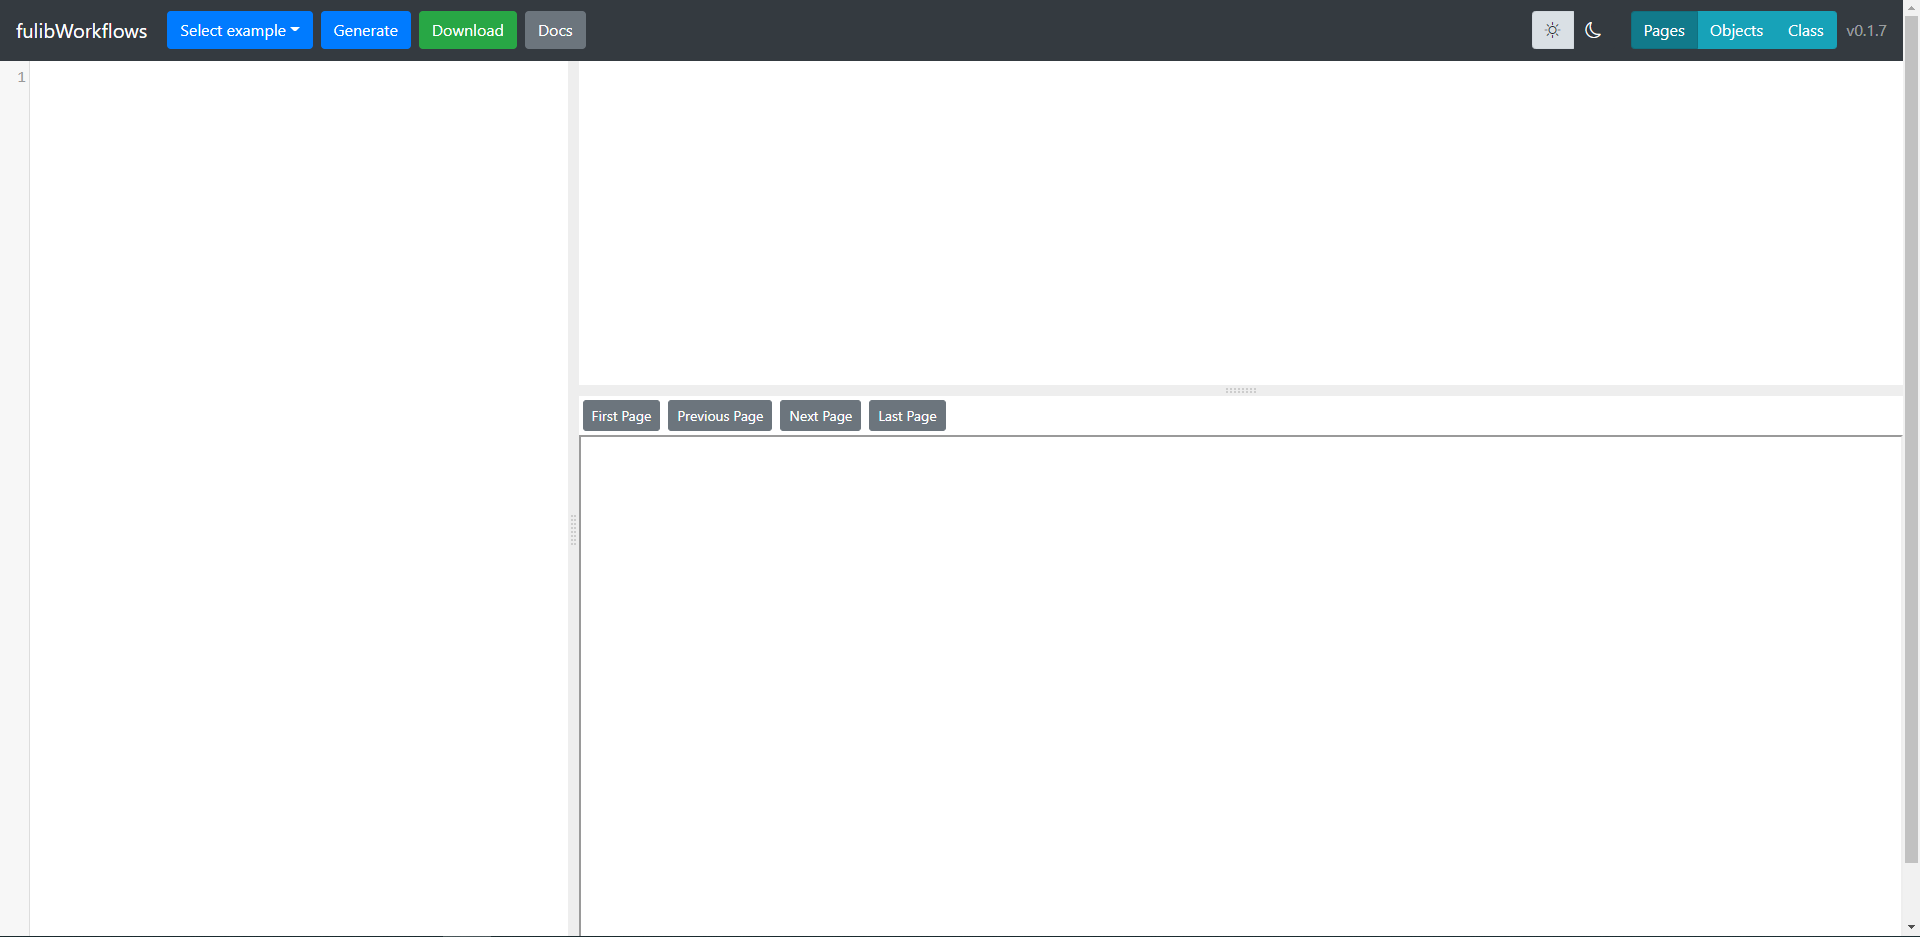
\includegraphics[width=1.0\textwidth]{images/3.2/workflows-complete}
    \caption{FulibWorkflows Web-Editor Oberfläche}
    \label{fig:frontend}
\end{figure}

In Abbildung~\ref{fig:frontend} ist die Oberfläche des Web-Editors dargestellt.
Dieser besteht aus vier verschiedenen Bereichen, welche jeweils andere Funktionen bereitstellen.
Der erste dieser Bereiche ist die Navigationsleiste, welche den oberen Rand der Oberfläche einnimmt.
In dieser steht zuerst, von links nach rechts, ein Dropdown Menü bereit, mit welchem es möglich ist verschiedene vorgefertigte Beispiele zu laden.
Diese Beispiele werden automatisiert nach der Auswahl ans Backend geschickt und dort generiert, sodass nach einer kurzen Wartezeit ein Event Storming Board und falls
vorhanden Mockups und Diagramme angezeigt werden können.
Als Nächstes folgt ein Knopf zum Anstoßen einer Generierung, nachdem dieser Knopf gedrückt wurde und die Generierung angestoßen ist, erscheint ein Ladekreis in dem Knopf,
um als Indikator dafür zu dienen, dass der Prozess noch nicht abgeschlossen ist.
Die Web-Anwendung ermöglicht es zusätzlich die in der Oberfläche erstellten Dateien herunterladen zu können.
Hierfür öffnet sich ein Pop-Up Bereich, nachdem der Download-Knopf betätigt wurde.
Dieses Fenster ist in Abbildung\ref{fig:download} dargestellt.

\begin{figure}[h]
    \centering
    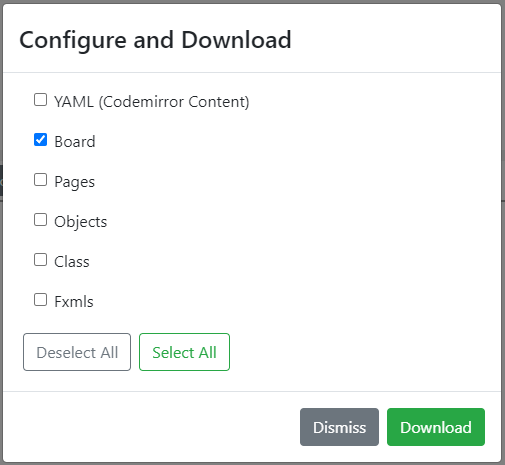
\includegraphics[width=0.5\textwidth]{images/3.2/download}
    \caption{Download Fenster}
    \label{fig:download}
\end{figure}

Im sich öffnenden Fenster erhält der Benutzende die Möglichkeit auszuwählen, welche Dateien heruntergeladen werden sollen.
Es können nur einzelne Dateien heruntergeladen werden, wie der Inhalt des Code-Editors, das generierte Event Storming Board oder aber alle Dateien
die durch die aktuelle Workflow-Beschreibung im Code-Editor generiert wurden.
Mit einem erneuten Klick auf den Download-Knopf, welcher sich neben dem Dismiss-Knopf befindet, wird eine Zip-Datei generiert und automatisch durch den jeweiligen Browser heruntergeladen.
Für den Fall, dass der Nutzende noch keine Erfahrungen mit der Syntax von fulibWorkflows gemacht hat, kann die Dokumentation, welche auf Englisch verfasst ist, mit einem Klick
auf den grauen Docs-Knopf geöffnet werden.
Die Dokumentation stammt aus dem GitHub-Repository von fulibWorkflows.
Im rechten Bereich der Navigationsleiste befinden sich zwei Buttons, welche das Theme des Code-Editors abändern, damit ist es möglich einen Light- oder Dark-Mode zum Schreiben
des Codes zu verwenden.
Daneben finden sich drei weitere Buttons, welche die Anzeige der generierten Dateien umschaltet.
Hierbei kann zwischen dem Anzeigen der Mockups(Pages), der Objektdiagramme oder des Klassendiagrammes umgeschaltet werden.
Letztlich befindet sich ganz recht die aktuelle Versionsnummer des gesamten Web-Editors.

\todo{Resizable View dank angular split, daran die vier bereiche erläutern: Editor, Board, Pages}


\subsection{Codeeditor}\label{subsec:codeeditor}

\todo{Grundlage ist CodeMirror, was für Addons wurden benutzt?, eigenes Add on erklären, wie wird die Eingabe validiert(ajv, schema)}

\subsection{Darstellung generierter Dateien}\label{subsec:darstellung-generierter-dateien}

\todo{Was macht der Iframe vom Board? Wie kann man von einem Iframe auf den anderen zugreifen(Parent functions)? Was kann der bereich der mockups/diagramme so mit den Buttons?}
